\section{Entraînement}
    Il a été décidé de faire l'entraînement des réseaux de neurones sur 10 époques, car l'entraînement doit être rapide dans un contexte d'entraînement en ligne et de génération d'un signal de curiosité utilisé dans un mécanisme d'attention. Une recherche d'hyperparamètres a été effectuée pour trouver la meilleur configuration de chaque modèle. Tous les modèles ont été entraînés sur les images d'entraînement pour chaque base de données.
    
\section{Résultats}
    Les sous-sections suivantes présentent les résultats obtenus. Les fonctions de coût d'entraînement ne peuvent pas être comparées entre les modèles, car leur plage dynamique n'est pas la même. Cependant, les métriques de validation et de test peuvent être comparées entre les modèles, car elles sont obtenues avec les données de validation et de test respectivement.

\subsection{Courbes d'apprentissage}
    Les courbes d'apprentissage ont été analysées pour s'assurer que l'apprentissage non supervisé permet d'améliorer la métrique de validation au fil de l'entraînement. Les figures \ref{fig:learning_curves_a}, \ref{fig:learning_curves_b}, \ref{fig:learning_curves_c}, \ref{fig:learning_curves_d} et \ref{fig:learning_curves_e} présentent des courbes d'apprentissage typiques pour les modèles A, B, C, D et E respectivement. L'entraînement non supervisé converge pour l'ensemble des modèles parce que les fonctions de coût de l'entraînement diminuent au fil des époques.\\

    À l'aide des courbes d'apprentissage des modèles A, B et C, il est possible de tirer que la métrique de validation est améliorée au fur et à mesure de l'entraînement. Par conséquent, il est possible de continue l'analyse de résultats pour ces modèles. Grâce à l'analyse des courbes d'apprentissage des modèles C et D, il est possible de conclure que la métrique de validation est détériorée au fil de  l'entraînement de ces modèles. Ceci est possiblement dû à ce qu'il n'y a aucun critère dans la fonction de coût d'entraînement pour permettre un bon entraînement des réseaux d'extraction des caractéristiques. La méthode d'entraînement de ces deux réseaux ne leur permet pas l'extraction de bonnes caractéristiques. Ainsi, les modèles C et D ne seront pas analysés plus en détail dans la suite du document.

    \begin{figure}[H]
        \centering
        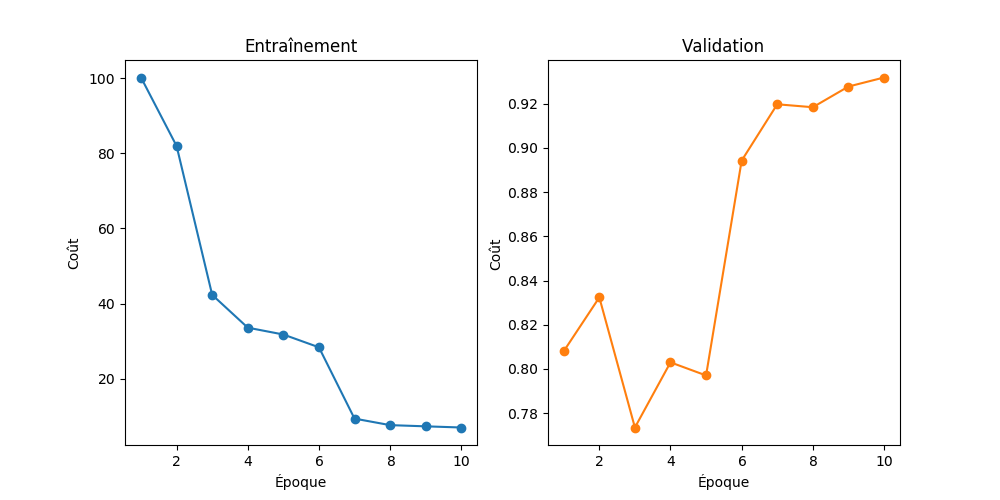
\includegraphics[width=16cm]{images/learning_curves_a.png}
        \caption{Exemple de courbe d'apprentissage du modèle A}
        \label{fig:learning_curves_a}
    \end{figure}

    \begin{figure}[H]
        \centering
        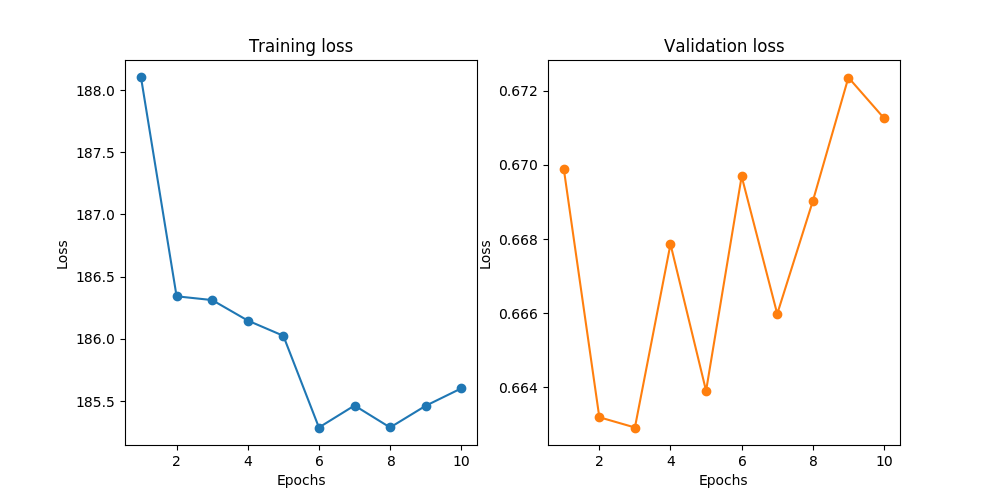
\includegraphics[width=16cm]{images/learning_curves_b.png}
        \caption{Exemple de courbe d'apprentissage du modèle B}
        \label{fig:learning_curves_b}
    \end{figure}

    \begin{figure}[H]
        \centering
        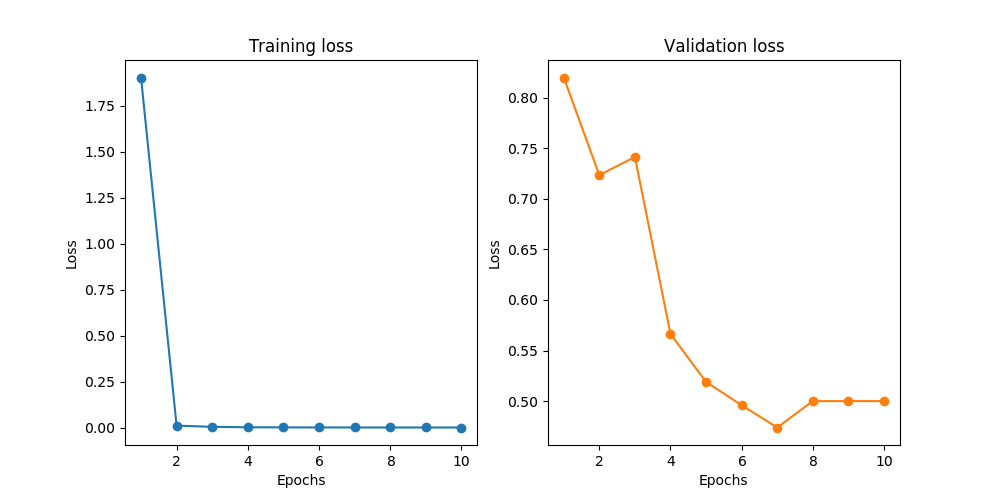
\includegraphics[width=16cm]{images/learning_curves_c.png}
        \caption{Exemple de courbe d'apprentissage du modèle C}
        \label{fig:learning_curves_c}
    \end{figure}

    \begin{figure}[H]
        \centering
        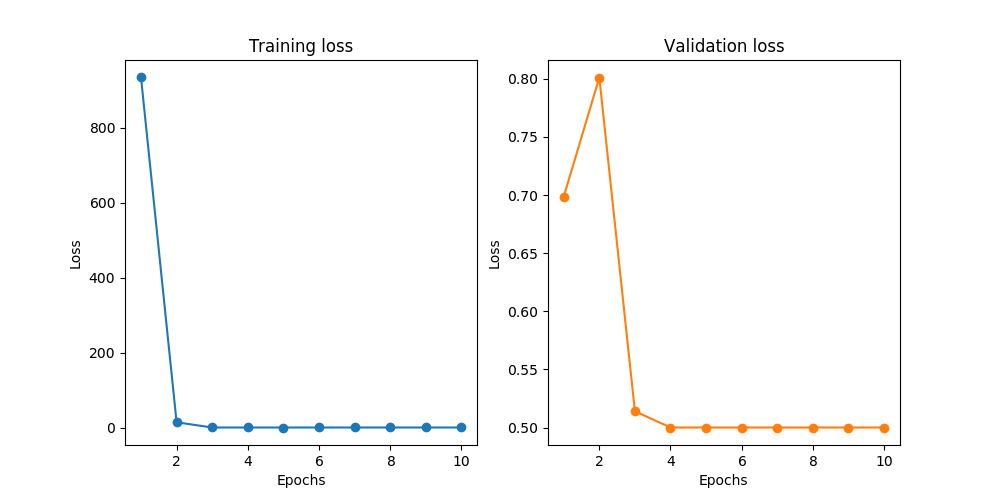
\includegraphics[width=16cm]{images/learning_curves_d.png}
        \caption{Exemple de courbe d'apprentissage du modèle D}
        \label{fig:learning_curves_d}
    \end{figure}

    \begin{figure}[H]
        \centering
        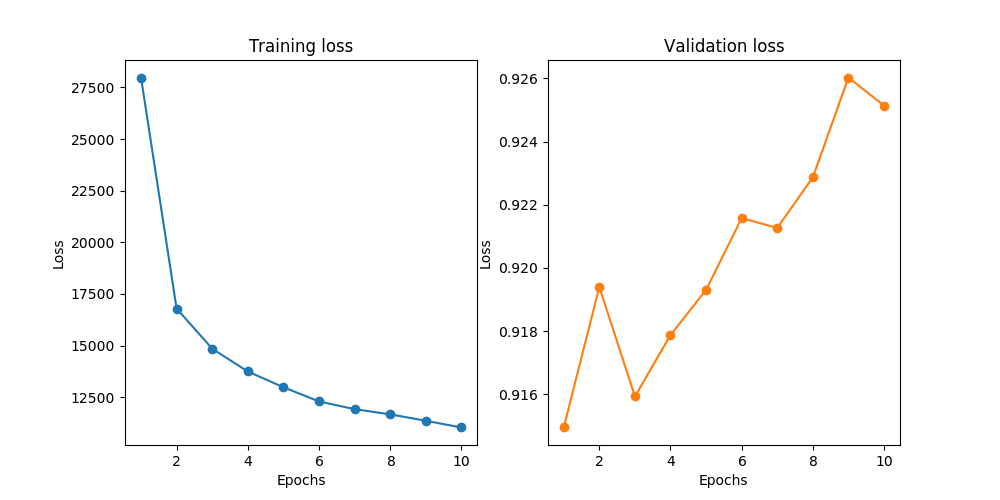
\includegraphics[width=16cm]{images/learning_curves_e.png}
        \caption{Exemple de courbe d'apprentissage du modèle E}
        \label{fig:learning_curves_e}
    \end{figure}

\subsection{Base de données - Tunnel}
    Une recherche d'hyperparamètres et des tests ont été effectués pour déterminer les meilleures configurations des modèles et le meilleur modèle sur la base de données tunnel.

\subsubsection{Recherche des hyperparamètres}
    Le tableau \ref{tab:resultat_tunnel_modele_a} présente les résultats de la recherche d'hyperparamètres pour le modèle A sur la base de données tunnel. Les configurations 5 à 10 donnent des performances sensiblement équivalentes, tandis que les performances des configurations 1 à 4 sont moins bonnes. Ces dernières sont les configurations donnant un modèle avec moins de paramètres. Alors, il est possible de conclure que le modèle doit avoir assez de paramètres pour avoir de bonne performance et que la meilleure configuration est la 8.
    
    \begin{table}[H]
        \centering
        \caption{Résultats de la recherche des hyperparamètres du modèle A - Tunnel}
        \label{tab:resultat_tunnel_modele_a}
        \begin{tabular}{lllp{3cm}p{3cm}l}
            \midrule
            \# & \(N_A\) & \(N_B\) & Augmentation des données & Métrique de validation & Époque\\
            \midrule\midrule
            1  & 2 & 2 & Non & 0,812 & 10\\
            2  & 2 & 2 & Oui & \\
            3  & 2 & 3 & Non & 0,614 & 1\\
            4  & 2 & 3 & Oui & 0,791 & 7\\
            5  & 4 & 2 & Non & 0,933 & 7\\
            6  & 4 & 2 & Oui & 0,932 & 10\\
            7  & 4 & 3 & Non & 0,930 & 7\\
            \textbf{8}  & \textbf{4} & \textbf{3} & \textbf{Oui} & \textbf{0,936} & \textbf{10}\\
            9  & 8 & 2 & Non & 0,934 & 4\\
            10 & 8 & 2 & Oui & 0,935 & 10\\
            \midrule
        \end{tabular}
    \end{table}

    Les résultats de la recherche des hyperparamètres du modèle B sont présentés dans le tableau \ref{tab:resultat_tunnel_modele_b}. L'ensemble des configurations donne des résultats semblables, mais la meilleure configuration est la 6.

    \begin{table}[H]
        \centering
        \caption{Résultats de la recherche des hyperparamètres du modèle B - Tunnel}
        \label{tab:resultat_tunnel_modele_b}
        \begin{tabular}{lllp{3cm}p{3cm}l}
            \midrule
            \# & \(N_A\) & \(N_B\) & Augmentation des données & Métrique de validation & Époque\\
            \midrule\midrule
            1  & 2 & 2 & Non & 0,612 & 9\\
            2  & 2 & 2 & Oui & 0,673 & 10\\
            3  & 2 & 3 & Non & 0,634 & 1\\
            4  & 2 & 3 & Oui & 0,673 & 6\\
            5  & 4 & 2 & Non & 0,613 & 6\\
            \textbf{6}  & \textbf{4} & \textbf{2} & \textbf{Oui} & \textbf{0,673} & \textbf{2}\\
            7  & 4 & 3 & Non & 0,621 & 4\\
            8  & 4 & 3 & Oui & 0,672 & 9\\
            9  & 8 & 2 & Non & 0,632 & 2\\
            10 & 8 & 2 & Oui & 0,672 & 6\\
            \midrule
        \end{tabular}
    \end{table}

    Le tableau \ref{tab:resultat_tunnel_modele_e} permet de constater que l'entraînement du \textit{backend} VGG16 cause une détérioration significative des performances. Ceci est possiblement relié à la détérioration des performances de validation au fil de l'entraînement des modèles C et D. Lorsqu'il y a entraînement du \textit{backend} VGG16, l'extraction des caractéristiques est détériorée, car la méthode d'entraînement ne permet pas l'apprentissage de ceci. La meilleure configuration est la 1.

    \begin{table}[H]
        \centering
        \caption{Résultats de la recherche des hyperparamètres du modèle E - Tunnel}
        \label{tab:resultat_tunnel_modele_e}
        \begin{tabular}{lp{3cm}p{3cm}p{3cm}l}
            \midrule
            \# & Entraînement du \text{backend} & Augmentation des données & Métrique de validation & Époque\\
            \midrule\midrule
            \textbf{1} & \textbf{Non} & \textbf{Non} & \textbf{0,931} & \textbf{10}\\
            2 & Non & Oui & 0,926 & 9\\
            3 & Oui & Non & 0,500 & 8\\
            4 & Oui & Oui & 0,500 & 8\\
            \midrule
        \end{tabular}
    \end{table}

\subsubsection{Comparaison entre les modèles}
    Les meilleures configurations des modèles A, B et E ont été testé sur les images de test de à base de données tunnel. Les courbes ROC présentées à la figure \ref{fig:tunnel_roc} ont été obtenues à partir de ces tests. Une autre métrique de comparaison intéressante pour comparer les différents modèles est le temps d'exécution. Le tableau \ref{tab:resultat_tunnel_temps_execution} présente les temps d'exécution moyens pour la passe avant, la passe arrière et total pour chacun des modèles sur une carte Tesla K20. À partir de ces informations, il est possible de conclure que le meilleur modèle pour cette base de données est le E parce que l'aire sous la courbe ROC est la plus grande et que son temps d'exécution est le moins élevé. À partir de ces résultats, il est possible d'invalider l'hypothèse énoncée par rapport à l'auto-encodeur variationnel (modèle B). Le fait de contraindre la sortie de l'encodeur détériore les performances que ce soit pour la courbe ROC ou pour le temps d'exécution.
    
    \begin{figure}[H]
        \centering
        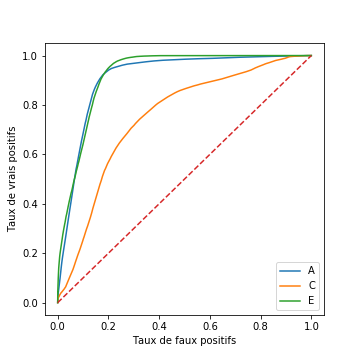
\includegraphics[width=8cm]{images/tunnel_roc.png}
        \caption{Courbes ROC - Tunnel}
        \label{fig:tunnel_roc}
    \end{figure}

    \begin{table}[H]
        \centering
        \caption{Temps d'exécution moyens sur Tesla K20 - Tunnel}
        \label{tab:resultat_tunnel_temps_execution}
        \begin{tabular}{lp{4cm}p{4cm}p{4cm}}
            \midrule
            Modèle & Temps d'exécution moyen de la passe avant (ms) & Temps d'exécution moyen de la passe arrière (ms) & Temps d'exécution total moyen (ms)\\
            \midrule\midrule
            A & 2,93 & 4,75 & 7,68\\
            B & 3,65 & 5,86 & 9,51\\
            E & 3,14 & 2,78 & 5,92\\
            \midrule
        \end{tabular}
    \end{table}

\subsection{Base de données - Faculté de génie}

\subsubsection{Recherche des hyperparamètres}
    \begin{table}[H]
        \centering
        \caption{Résultats de la recherche des hyperparamètres du modèle A - Faculté de génie}
        \label{tab:resultat_corridor_modele_a}
        \begin{tabular}{lllp{3cm}p{3cm}l}
            \midrule
            \# & \(N_A\) & \(N_B\) & Augmentation des données & Métrique de validation & Époque\\
            \midrule\midrule
            1  & 2 & 2 & Non & 0,501 & 1\\
            2  & 2 & 2 & Oui & 0,610 & 7\\
            3  & 2 & 3 & Non & 0,665 & 8\\
            4  & 2 & 3 & Oui & 0,644 & 10\\
            \textbf{5}  & \textbf{4} & \textbf{2} & \textbf{Non} & \textbf{0,678} & \textbf{10}\\
            6  & 4 & 2 & Oui & 0,652 & 10\\
            7  & 4 & 3 & Non & 0,677 & 10\\
            8  & 4 & 3 & Oui & 0,666 & 7\\
            9  & 8 & 2 & Non & 0,667 & 9\\
            10 & 8 & 2 & Oui & 0,672 & 10\\
            \midrule
        \end{tabular}
    \end{table}
    
    \begin{table}[H]
        \centering
        \caption{Résultats de la recherche des hyperparamètres du modèle B - Faculté de génie}
        \label{tab:resultat_corridor_modele_b}
        \begin{tabular}{lllp{3cm}p{3cm}l}
            \midrule
            \# & \(N_A\) & \(N_B\) & Augmentation des données & Métrique de validation & Époque\\
            \midrule\midrule
            1  & 2 & 2 & Non & 0,499 & 7\\
            2  & 2 & 2 & Oui & 0,503 & 5\\
            3  & 2 & 3 & Non & 0,499 & 10\\
            4  & 2 & 3 & Oui & 0,502 & 4\\
            \textbf{5}  & \textbf{4} & \textbf{2} & \textbf{Non} & \textbf{0,511} & \textbf{1}\\
            6  & 4 & 2 & Oui & 0,501 & 10\\
            7  & 4 & 3 & Non & 0,501 & 8\\
            8  & 4 & 3 & Oui & 0,500 & 2\\
            9  & 8 & 2 & Non & 0,499 & 1\\
            10 & 8 & 2 & Oui & 0,501 & 10\\
            \midrule
        \end{tabular}
    \end{table}
    
    \begin{table}[H]
        \centering
        \caption{Résultats de la recherche des hyperparamètres du modèle E - Faculté de génie}
        \label{tab:resultat_corridor_modele_e}
        \begin{tabular}{lp{3cm}p{3cm}p{3cm}l}
            \midrule
            \# & Entraînement du \text{backend} & Augmentation des données & Métrique de validation & Époque\\
            \midrule\midrule
            \textbf{1} & \textbf{Non} & \textbf{Non} & \textbf{0,719} & \textbf{10}\\
            2 & Non & Oui & 0,699 & 7\\
            3 & Oui & Non & 0,500 & 10\\
            4 & Oui & Oui & 0,500 & 10\\
            \midrule
        \end{tabular}
    \end{table}

\subsubsection{Comparaison entre les modèles}
    \begin{figure}[H]
        \centering
        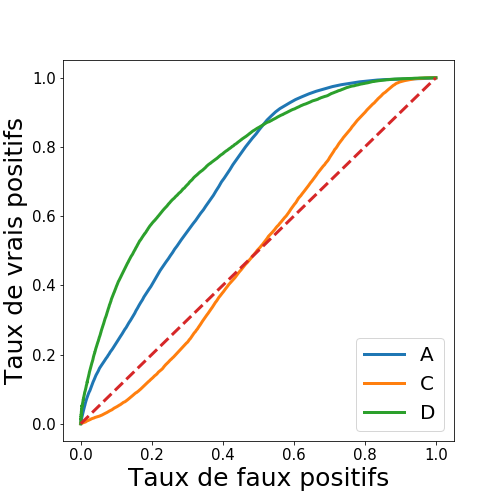
\includegraphics[width=8cm]{images/corridor_roc.png}
        \caption{Courbes ROC - Faculté de génie}
        \label{fig:corridor_roc}
    \end{figure}

    \begin{table}[H]
        \centering
        \caption{Temps d'exécution moyens sur Tesla K20 - Faculté de génie}
        \label{tab:resultat_corridor_temps_execution}
        \begin{tabular}{lp{4cm}p{4cm}p{4cm}}
            \midrule
            Modèle & Temps d'exécution moyen de la passe avant (ms) & Temps d'exécution moyen de la passe arrière (ms) & Temps d'exécution total moyen (ms)\\
            \midrule\midrule
            A & 3,08 & 4,22 & 7,30\\
            B & 3,65 & 5,86 & 9,51\\
            E & 3,14 & 2,78 & 5,92\\
            \midrule
        \end{tabular}
    \end{table}

\subsection{Analyse générale}
    